\documentclass[12pt, a4paper, twoside]{book} % book style
\usepackage[portuges, english]{babel} % hyphenation (english is the default)
\usepackage[utf8]{inputenc} % allow utf-8 characters
\usepackage[T1]{fontenc} % T1 font encoding
\usepackage[scaled]{beramono} % Bitstream Vera (used in code listings)
\usepackage[babel, tracking, spacing, kerning]{microtype} % enhanced typography
\usepackage{setspace} % provides \onehalfspacing
\usepackage{quotchap} % pretty chapter headers
\usepackage[pdfpagelabels]{hyperref} % PDF hyperlinks
\usepackage[all]{hypcap} % fix hyperref caption problem
\usepackage{pdfpages} % include pdf pages (for the cover)
\usepackage{listings} % for the source code
\usepackage{booktabs} % pretty tables, provides \toprule \midrule \bottomrule
\usepackage{graphicx}
%\usepackage{asmath}
%\usepackage{assymb}
\usepackage{txfonts}% use Arial && Times New Roman
\usepackage{epigraph}
\usepackage{subfigure}
% \usepackage{amssymb}
\usepackage{todonotes}

\setlength{\oddsidemargin}{31.0pt}
\setlength{\evensidemargin}{31.0pt}
% change quotchap chapter number to black
\definecolor{chaptergrey}{rgb}{0,0,0}

% reduce vertical spacing of quotchap chapter heading
\let\defaultchapterheadstartvskip\chapterheadstartvskip
\makeatletter
\renewcommand*\chapterheadstartvskip{
  \if@mainmatter % but only in the main matter
    \vspace*{-3.0\baselineskip}
  \else
    \defaultchapterheadstartvskip
  \fi
}
\makeatother

% set line spacing to 1.5
\onehalfspacing

% setup hyperref and set pdf metadata
\hypersetup{
    pdftitle   = {Opportunistic Privacy Preserving Bluetooth Sensing},
    pdfauthor  = {Nelson Gonçalves PG15395},
    colorlinks = false,
    hidelinks
}

% listing style for Python code
\lstdefinestyle{Python Code}{
	language=Python,
  	tabsize=4,
  	commentstyle=\itshape,
  	basicstyle=\ttfamily\small,
  	frame=single,
  	numbers=left,
    numberstyle=\ttfamily\small,
    lineskip=-1.5pt,
}

% abstract environment
\newenvironment{abstract}
{\cleardoublepage \thispagestyle{plain} \null \vfill
\begin{center} \bfseries \abstractname \end{center}}
{\vfill \null}

% acknowledgements environment
\addto\captionsenglish{\def\ackname{Acknowledgements}} % ackname in english
\addto\captionsportuges{\def\ackname{Agradecimentos}} % ackname in portuguese
\newenvironment{acknowledgements}
{\cleardoublepage \thispagestyle{plain} \null \vfill
\begin{center} \bfseries \ackname \end{center}}
{\vfill \null}

%-----------------------------------------------------------------------------%

\begin{document}
\pagestyle{empty}
% Cover
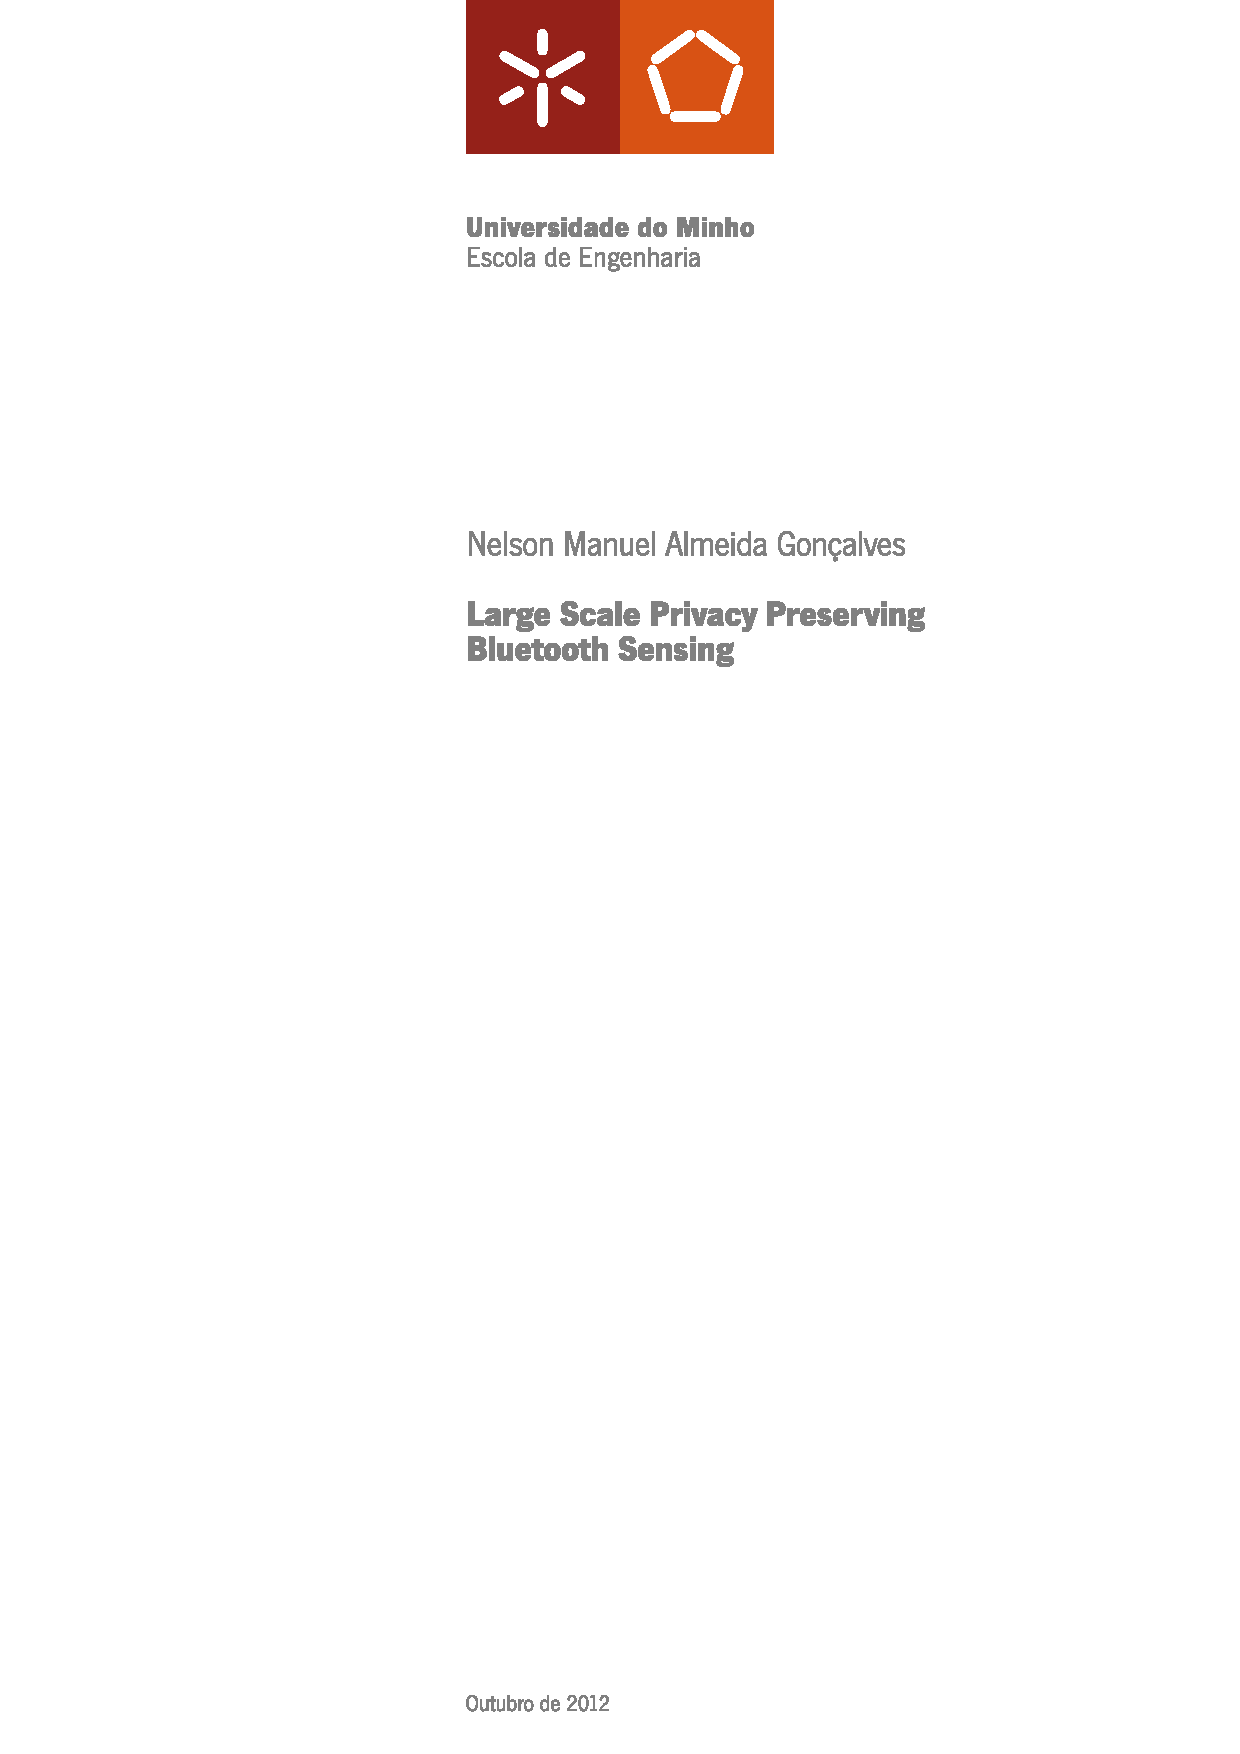
\includepdf[pages=1]{images/cover.pdf}
\selectlanguage{portuges}

\noindent{\LARGE\textbf{Declaração}}
\par\vspace{10mm}
\noindent{\textbf{Nome:}} Nelson Manuel Almeida Gonçalves
\par\vspace{3mm}
\noindent{\textbf{Endereço Electrónico:}} goncalvesnelson@gmail.com
\par\vspace{3mm}
\noindent{\textbf{Telefone:}} 937528319
\par\vspace{3mm}
\noindent{\textbf{Bilhete de Identidade:}} 13220550
\par\vspace{3mm}
\noindent{\textbf{Título da Tese:}} Large Scale Privacy Preserving Bluetooth Sensing
\par\vspace{3mm}
\noindent{\textbf{Orientador:}} Doutor Carlos Miguel Ferraz Baquero Moreno
\par\vspace{3mm}
\noindent{\textbf{Co-Orientador:}} Doutor Rui João Peixoto José
\par\vspace{3mm}
\noindent{\textbf{Ano de conclusão:}} 2012
\par\vspace{3mm}
\noindent{\textbf{Designação do Mestrado:}} Mestrado em Engenharia Informática
\par\vspace{20mm}
\noindent{É AUTORIZADA A REPRODUÇÃO INTEGRAL DESTA TESE APENAS PARA
EFEITOS DE INVESTIGAÇÃO, MEDIANTE DECLARAÇÃO ESCRITA DO
INTERESSADO, QUE A TAL SE COMPROMETE.}
\par\vspace{10mm}
\begin{center}
Universidade do Minho, 31 de Dezembro de 2012
\par\vspace{3mm}
Nelson Manuel Almeida Gonçalves
\end{center}
 % Permissao

\selectlanguage{english}
\cleardoublepage

\newpage
% Epígrafe
\vspace*{0.8\textheight} \setlength{\epigraphwidth}{9cm}
\renewcommand{\textflush}{flushright} \epigraph{It suddenly struck me
  that that tiny pea, pretty and blue, was the Earth. I put up my
  thumb and shut one eye, and my thumb blotted out the planet Earth. I
  didn’t feel like a giant. I felt very, very small.}
{Neil Armstrong}

\cleardoublepage
% Front matter
\frontmatter
\pagestyle{headings}
% vim: set ts=4 sw=4 ai et tw=74:
\chapter*{}
\begin{center}\textbf{Acknowledgements}\end{center}
	
I would like to express my special gratitude to Professor Carlos Baquero, for being my advisor and supporting my work with great advise and encouragement, through the last several months. Also a special thanks to Professors Paulo Sérgio Almeida and Vítor Fonte, both heavily involved in this project. Without forgetting Nuno Preguiça from \emph{Universidade Nova de Lisboa}, the consulter of this project. To all of them, thank you for the continuous support and encouragement throughout this work and for the counseling provided. I learned a lot. Without their guidance and dedication this dissertation would not have been possible.\\
Thanks to my colleagues and friends at the laboratory, for the pleasant environment created. Thanks to Pedro Gomes for the exchange of ideas and brainstorming that we often had. It was of great value.\\
Additionally, I am grateful to my family and Ana, for all the love and support given, and for always having confidence in me.\\
Finally, a special thanks to \emph{Fundação para a Ciência e a Tecnologia (FCT)} for supporting this work through project CASTOR (Causality Tracking for Optimistic Replication in Dynamic Distributed Systems), under Research Grant (BI) number: BI1-2010\_PTDC/EIA-EIA/104022/2008\_UMINHO



\thispagestyle{empty}
 % Acknowledgments

\selectlanguage{portuges}

%%% Local Variables: 
%%% mode: latex
%%% TeX-master: "thesis"
%%% End: 
 % Resumo
\selectlanguage{english}

%%% Local Variables: 
%%% mode: latex
%%% TeX-master: "thesis"
%%% End: 
 % Abstract

\tableofcontents
\listoffigures
\addcontentsline{toc}{chapter}{\listfigurename}
% \listoftables
% \addcontentsline{toc}{chapter}{\listtablename}

% Main matter
\mainmatter
\chapter{Introduction}
\label{cha:introduction}

Propelled by the increasing usage of web enabled, context and location
aware mobile devices, context aware services specially location based
services (LBS) are becoming remarkably popular. The recent
developments seen in technologies like GPS, GSM, Wifi and Bluetooth
also worked as a catalyst in this process. Using these technologies it
is possible to obtain information about the location of users. This
type of information can be used both by service providers and
users. Service providers can process this information to obtain a
better understanding of the users behavior (e.g. by analyzing their
movement) and improve their current services, as well as plans for
future services and infrastructures. Users, on the other hand, can use
location data to get personalized information according to their
location. However, the continuous monitoring, processing and storage
of location data can create privacy related problems. Location
information can expose sensitive information about users as it
constitutes a \emph{quasi-identifier}\footnote{Data that by itself
  does not uniquely identify a user but that in association with other
  information might.} according to Bettini et
al.~\cite{bettini2005protecting}.

Examples of attacks on privacy using recorded location data are not
hard to find. Using a week-long database, with GPS traces of Detroit
drivers whose names were replaced with pseudonyms, Hoh et
al.~\cite{hoh2006enhancing} were able to determine the location of
85\% of the drivers' homes. Hightower et al.'s BeaconPrint
algorithm~\cite{hightower2005learning} is able to accurately recognize
the location of a user using only Wifi and GSM
information. Researchers have also shown that, looking at the historic
of someone's location data, it is possible to predict their future
whereabouts~\cite{krumm2006predestination,froehlich2008route}.

While location based information is very useful, the fact that it can
be used to attack the privacy of the users might be a decisive factor
in the popularity and sustainability of services supported by this
type of information.  The solution to this problem consists in the use
of privacy preserving approaches capable of ensuring both the quality
of the service and the privacy of its users.

Stochastic summarizing techniques are space efficient, probabilistic
mechanisms, capable of producing summaries of the data they receive as
input.  The size of the summaries depends only on the number of input
elements, not on the size of the elements. Being non-deterministic,
these techniques do not allow the original item to be recreated from
its resulting summary. However they do offer a trade-of between space
and accuracy where one is obtained at the expense of the other.

% i.e., it is always $x * N$ bits, where $x$ is a
% predetermined value and $N$ is the number of elements

This dissertation aims to find if stochastic summarizing techniques
are suitable as privacy preserving techniques regarding location
data in large scale scenarios. As a proof of concept, we present two
Bluetooth based scenarios, where we make use of these techniques
to ensure the privacy of the users while trying to comply with the
scenarios' requirements.

Bluetooth technology is a relatively easy and inexpensive way to track
large groups of people. Unlike technologies like GPS, Bluetooth also
works well in both indoors and outdoors scenarios. This allows the
tracking of individuals both inside and outside buildings allowing for
more robust tracking solutions.  Also, Bluetooth has a limited
detection range (typically between 10 to 100 meters depending on the
number of obstacles) which makes the differentiation between nearby places
possible, thus enabling accurate tracking results. Furthermore,
Bluetooth tracking is a passive tracking process, i.e, it does not
require users to change their behavior. On the other hand, GPS
positions are computed in the mobile device and have to be handed to
the tracking entity.  All these properties make Bluetooth an arguably
good choice in which to base our tracking scenarios.

As Bluetooth becomes more and more pervasive, there is a growing
potential to leverage on the possibilities offered by Bluetooth
scanning as a flexible infrastructure for situated interaction and a
general purpose platform for massive sensing and actuation in physical
spaces.

Bluetooth sensing is based on a discovery process through
which a device can inquire about the presence of other nearby devices.
If those devices are in \emph{discoverable} mode, they will respond
with their Bluetooth addresses (48 bit MAC), and possibly additional
information, such as the device name, the device type (e.g. cellphone
or computer) and available services.

A Bluetooth scanner is a device that periodically scans nearby
Bluetooth devices. Each time a device is detected, it registers and
timestamps that event. Later, this information can be used by external
services or applications. Multiple Bluetooth scanners spread all over
a physical space could thus serve as collection points for Bluetooth
sightings, providing a major tool for observing, recording, modeling
and analyzing that space, physically, digitally and socially
\cite{Oneill:2006vq}.

An infrastructure of this nature can be built from scratch given
the increasingly smaller cost of the technological equipment required.
Alternatively, it can be built upon the large number of Bluetooth
scanners already present in some urban environments. These scanners
are owned by many entities and they serve very diverse purposes, such
as proximity marketing, device localization or OBEX-based interaction.
They could be used, without any additional cost, as nodes in a large
scale collaborative sensing infrastructure. Each node would still scan
for its own purposes, but it would also share part of the generated
data with a central service that would then be able to produce
aggregate information of mutual interest. Both strategies make the
creation of this type of infrastructure relatively simple and feasible
in the short term.

The challenge, however, is how to enable this type of large scale
sensing without creating an overwhelming privacy threat to the users.

% There are already several techniques whose purpose is to ensure
% location privacy in the exchange of information between users and
% service providers. This dissertation aims to find if stochastic
% summarizing techniques are suitable as building blocks for privacy
% preserving systems. To assess their viability, we used them in two
% different Bluetooth scanning scenarios.

\section{Structure and Contributions}
\label{sec:structure}

\subsubsection{Structure}
\label{sec:structure} This dissertation is organized as follows:
Chapter \ref{chap:literature_review} presents some of the related work
in the field of location privacy followed by a brief description of
some algorithms/data structures used in our privacy preserving
approaches. Chapters \ref{cha:gate-counting} and
\ref{cha:causality-tracking} describe both our Bluetooth tracking
scenarios, Collaborative Gate Counting and Causality Tracking, their
requirements and the effectiveness of several stochastic summarizing
techniques in dealing with them. Chapter \ref{cha:conclusion} draws
some general conclusions about our work and presents some future
research directions to be followed.

\subsubsection{Contributions}
\label{sec:contributions}
As a result of the work developed in the context of this dissertation,
two full papers were written. The first one
\cite{gonccalves2011privacy} was published in the OTM 2011 Workshop Proceedings.
The second paper \cite{inforum2012} was published in INFORUM 2012
where it was awarded the prize for best paper in the Mobile and
Ubiquitous Computing session.

%%% Local Variables:
%%% mode: latex
%%% TeX-master: "../thesis"
%%% End:
 % Introduction
\chapter{Literature Review}
\label{chap:literature_review}

This chapter exposes some of the works whose content is relevant to
the context of this dissertation. Section
\ref{sec:privacy_pervasive_computing} begins by explaining the concept
of location privacy in pervasive computing and it's importance. It then follows
with the presentation of some of the approaches already used in the
ofield of pervasive computing regarding this topic. Lastly, Section
\ref{sec:algorithms_and_data_structures} provides some background to
the algorithms and classic data structures used in our approach to ensure
privacy.
\section{Location Privacy in Pervasive Computing}
\label{sec:privacy_pervasive_computing}

\subsection{Definition of Location Privacy}
\label{sec:definition_privacy}
As location based services become more popular and compelling, there
is an increasing temptation to give away location data. However, along
with this temptation comes an increasing concern about location
privacy.

Beresford and Stajano ~\cite{1186725} define location privacy as:
\begin{quotation}
  ...the ability to prevent other parties to from learning one's
  current or past location.
\end{quotation}
Their definition implies that a person whose location is being
monitored must be able to control who has access that information.
It also acknowledges that both past and present information regarding location
are important. While current location information might enable an
attacker to find out where a person is, past data can allow him/her to
discover who the person is and where does she live/work among other
things.

According Duckham and Kulik~\cite{duckham2006location} location
privacy is:
\begin{quotation}
  a special type of information privacy which concerns the claim
  of individuals to determine for themselves when, how, and to what
  extent location information about them is communicated to others.
\end{quotation}
Their definition is based upon Westin's~\cite{westin1968privacy}
definition of information privacy:
\begin{quotation}
  the claim of individuals, groups or institutions to determine for
  themselves when, how and to what extent information about them is
  communicated to others.
\end{quotation}
Duckham and Kulik's definition captures several aspects about
location information and the way it can be shared:
\begin{itemize}
\item When: A user might have different concerns regarding her present
  and past locations. For instance, the user may not care as much
  about revealing her past locations as it does about its present
  location.
\item How: A user might be comfortable with manual location requests
  from her friends, however she may not want to have her friends
  alerted automatically when she enters a casino or a bar.  
\item Extent: A user might prefer to have her location reported as an
  ambiguous region rather than as a precise point.
\end{itemize}
These different aspects are the topic of many different
computational schemes for protecting the privacy of the users.
Examples of such schemes are the use of pseudonyms instead of actual
names, the deliberate addition of noise to the location data or the use
of regions for location reporting instead of specific points.

\subsection{Related Work}
\label{sec:lp_related_work}

% In the context of ubiquitous computing, there are already several
% techniques aimed at ensuring the privacy of data regarding the
% location of the users.

In the past few years there has been an exponential increase in the
number of mobile devices (smartphones, laptops, tablets). Many of
these devices come equipped with several types of sensors
(accelerometer , gyroscope, thermometer, GPS) as well as communication
interfaces (Bluetooth, WiFi). Their pervasiveness associated with
their capabilities make them viable building blocks for urban
pervasive infrastructures~\cite{kostakos2009understanding}. Associated
with the increasing number of mobile devices is the popularity growth
of Location-Based Services (LBS)\cite{zickuhr2012three}. LBSs
determine the location of the user by using one of several
technologies for determining position, and then use the location and
other information to provide personalized applications and
services~\cite{zibuschka2011location}. There are however privacy risks
that stem from the use of such services.
PleaseRobMe\footnote{pleaserobme.com} was created to raise awareness
for the risks of sharing location information. Combining information
from FourSquare\footnote{https://foursquare.com/} and
Twitter\footnote{www.twitter.com} it demonstrates how easy it is to
infer that someone is not at home. Despite the existence of reports
linking the sharing of location information with the occurrence of
robberies\cite{Grove:2009:Online,Dybwad:2009:Online}, there are
several research works that show that most people put little value on
their location privacy~\cite{ahern2007over,colbert2001diary,
  Cvrcek:2006:SVL:1179601.1179621,kaasinen2003user}. However, this
lack of concern by the users of LBSs is usually a consequence of lack
of awareness. In \cite{kaasinen2003user} the author notes that,
despite not being worried about the privacy issues with location aware
services, most of the users were not aware they could be located while
using those services. On the other hand, the work in
\cite{Cvrcek:2006:SVL:1179601.1179621} shows that the Greeks demanded
a higher price for their location data when compared with the other EU
countries. According to the author, this might have been a consequence
of the eavesdropping scandal involving the wiretap of Greek
politicians that took place 2 months before the survey. This might
indicate that people value their privacy the most when faced with
consequences from the lack of it. Sharing location data at such a
large scale like we see today is relatively new. As a consequence the
effects on user privacy are not fully understood
yet \cite{Terrovitis:2011:PPD:2031331.2031334}.

According to Duckham and Kulik survey in \cite{duckham2006location},
there are four commonly used methods for ensuring location privacy:
\begin{itemize}
\item Regulatory strategies: comprised by government rules on the use
  of personal information.
\item Privacy Policies: trust-based mechanisms established
  between individuals and whomever is receiving their location data.
\item Anonymity: Disassociation between the individual's personal
  information and individual's actual identity. Usually obtained through
  the use of pseudonyms,ambiguity and cloaking.
\item Obfuscation: degradation of the quality of the location data.
\end{itemize}

From these four methods, we will concentrate in the last two because
they are the most relevant in the context of this dissertation.

\subsubsection{Anonymity}
\label{sec:privacy_anonimity}

The use of pseudonyms is perhaps the most obvious way to achieve
anonymity. However, using same pseudonym for a long time makes it is
easy for an attacker to gather enough history on an individual to
infer their habits or true identity. To try to mitigate this issue,
Beresford and Stajano in \cite{1186725} proposed an idea which relied
upon pseudonym exchange. They introduced two new concepts: \emph{mix
  zone} and \emph{application zone}. A \emph{mix zone} for a group of
people is defined as the maximum contiguous area where none of the
group's users exchanges information with a LBS. This prevents the
users' data from being accessed by the LBSs providers. By contrast, an
\emph{application zone} is defined as an area where at least one of
the users exchanges data with a LBS. By switching her pseudonym to a
new unused one when entering a \emph{mix zone}, the user ensures that
there is no way for a LBS provider to distinguish between her and the
other users who were in that zone. This means that there is no way for
attackers to link people going into the mix zone with the ones that
come out of it.

Based on a different concept, \emph{k-anonymity} (introduced by
Samarati and Sweeney in~\cite{samarati1998protecting}) Gruteser and
Grunwald~\cite{gruteser2003anonymous} were the first to investigate
anonymity as a method to attain location privacy. According to them, a
subject is considered to be k-anonymous with regard to location
information, if and only if she is indistinguishable from at least
$k-1$ other subjects with respect to a set of
\emph{quasi-identifier}\footnote{Data that by itself does not uniquely
 identify a user but that in association with other
 information might}
attributes. Bigger values of $k$ correspond to higher degrees of
anonymity. They proposed a middleware architecture and an algorithm
capable of adjusting location information resolution in spacial and/or
temporal dimensions in order to comply with a specific
\emph{k-anonymity} requirement. When a client requests a service,
their algorithm calculates a \emph{cloaking box/region} that contains
that client along with at least $K-1$ other users. That box is then
used as the client's location to request the service. If that box's
resolution is to coarse for some services, temporal cloaking can be
applied by delaying the user's service request. When more users come
near the client, a smaller cloaking region can be computed. This concept
has since been explored and improved in other scientific works.

Geddik and Liu's
\emph{ClickCloak} algorithm
~\cite{gedik2005location,gedik2008protecting} allows each user to
define her own minimum acceptable value for $k$ ($k_{min}$), as well
as the maximum acceptable values for temporal and spacial resolution.
Furthermore, they created an efficient message perturbation engine
capable of performing the location anonymization of users' requests.
This is accomplished by removing the users' identities from the
requests and with the use of spatiotemporal obfuscation of the
location information. 

Mokbel et al. in~\cite{mokbel2006new} use the \emph{k-anonymity} concept as well.
They present the Casper framework which consists of two main
components, a location anonymizer and a privacy-aware query processor.
The location anonymizer blurs the location information about each user
according to that user's defined preferences (minimum area $A_{min}$
in which she wants to hide and minimum value for $k$). The query
processor tunes the functionality of traditional location-based
databases to be privacy-aware. It does so by returning cloaked areas
instead of exact points when queried for location information.

Unlike the previous \emph{k-anonymity} based approaches that require a
centralized trusted server (Anonymizer) in order to compute the cloaking
regions, Ghinita et al. in ~\cite{ghinita2007prive} use a
decentralized peer-to-peer approach. This fixes two issues inherent to
the centralized server approach: 
\begin{itemize}
\item Fault Tolerance -  the
anonymizer is a single point of failure and the system cannot work
without it.
\item Security - all requests must go through the anonymizer, so in
  case it becomes compromised it would result in a serious security
  threat.
\end{itemize}
Their distributed protocol called PRIVÉ supports decentralized query
anonymization with load balancing and fault tolerance. In PRIVÉ, for a
user to be considered trustworthy and participate in the network she
needs a trust certificate obtained from a Certification Server. Users
in the network trust each other and communicate using a structured
peer-to-peer network. Users are grouped into clusters according to
their location. Each cluster has a leader which is recursively grouped
with other leaders to form other clusters with different leaders, just
like a B-Tree structure. This allows each user to create it's own
cloaking region by using information from other nearby users.
Furthermore, PRIVÉ also ensures \emph{reciprocity} in the creation of
cloaking regions. A cloaking region with $k$ users satisfies
reciprocity only if that same cloaking region is generated for each of
users. This means that an attacker cannot use \emph{minimality} attacks
\cite{wong2007minimality}, i.e. it cannot infer which user is the
source of the request with a probability bigger than $\frac{1}{k}$.

\subsubsection{Obfuscation}
\label{sec:Obfuscation}

Obfuscation based techniques usually degrade the ``quality'' of the
information in order to provide privacy protection. Even tough this may
seem comparable to what \emph{k-anonymity} based techniques, there is a
key difference. Obfuscation based techniques allow the actual identity
of the user to be revealed (thus making it suitable for applications
that require authentication or offer some sort of  personalization
\cite{langheinrich2001privacy}).

Duckam and Kulik
\cite{duckham2005formal} were the ones who introduced the idea of
obfuscation for location privacy. They talk about three distinct types of
imperfection that can be present in spacial information:
\begin{itemize}
\item Inaccuracy - lack of correspondence between information and
  reality. E.g. ``Braga is in Spain''
\item Imprecision - lack of specificity in the information. E.g.
  ``Braga is in Europe''
\item Vagueness - special type of imprecision that concerns the
  existence of indeterminate borderline
  cases~\cite{duckham2001formal}. E.g. ``Braga is in western Europe''.
  This is a vague statement since there is no clear definition about
  the borders of western Europe.
\end{itemize}

Any of these types of imperfection can be used to obfuscate an
individual's location. In this particular case, the authors use
imprecision to degrade the quality of the location information.
They adopt a discrete model for space representation through the use of
graphs. Geographic locations are modeled as a set of vertices $V$, and
the connectivity or adjacency between them is modeled as a set of
Edges $E$. A user's location is represented through a
vertex $l \in V$. Obfuscation is provided through the use of a group
of vertices $O$ such that $l \in O$ and $O \in V$, where for every
element $o \in O$, $o$ is \emph{indiscernible} from $l$. The larger
the set $O$, the less information is being revealed and therefore, the
greater is the individual's privacy. The set $O$ is used by their
algorithms to negotiate the balance between an individual's location
privacy and that individual's need for quality services. The more
information an individual is willing to reveal the higher the quality
of information he can provided with.

Another example of an obfuscation based approach is shown by
Ardagna et al. in ~\cite{ardagna2007middleware} and later improved in
\cite{ardagna2007location, ardagna2011obfuscation}. Their obfuscation
process allows users to express their privacy preferences using
another concept of theirs called \emph{relevance}. Relevance is a
value in the range $]0,1]$ and it represents the relative accuracy
loss in location measurement. It tends to 0 when the location
measurement is highly inaccurate and it is equal to 1 when the
location measurement achieves the best accuracy allowed by the
location technique in use. The higher the relevance the lower will be the
location privacy. Moreover, they define a set of basic
\emph{obfuscation operators} that are used to modify location
measurements. These operators can be further composed in order to
increase robustness against deobfuscation attacks and are
randomly selected and applied to the user's measured location ensuring
that the selected relevance value holds. This solution allows users to
abstract from both the obfuscation operators and the sensing
technology (Bluetooth, Wifi, GPS).

There are other examples of obfuscation approaches that are not only
oriented to location data but to the degradation of data in general
\cite{anciaux2008instantdb,heerde2006data}. In these approaches,
privacy is obtained through the generalization of the information.
This procedure is done resorting to generalization trees
\cite{anciaux2008instantdb} or generalization graphs
\cite{heerde2006data}. These structures contain the sets of rules to
be applied in the generalization process. The application of these
rules depends on the Life Cycle Policy (LCP). A LCP consists of the
set of transitions between the generalization structures'
branches/vertexes as well as the events that trigger them. The biggest
challenge in this type of approaches is the difficulty associated with 
the construction of the sets of rules and the generalization
structures.

% for self-protection, it is natural and necessary for a user to
% withhold her true identity when requesting an LBS. However, simply
% using a pseudonym, or not using any identifier at all, is not
% sufficient. This is due to the fact that a user’s location itself may
% be correlated with restricted spaces such as house and of- fice to
% reveal her real-world identity. For example, if a location belongs to
% a private property, then the adversary can derive that the user is
% most likely the owner of the property. A single loca- tion sample may
% not be linked directly to a particular user, but the accumulation of a
% time-series sequence of her location samples will eventually reveal
% her identity \cite{gruteser2005anonymity, xu2007location}. Once the
% user is identified, all her visits may be disclosed.

\section{Algorithms and data structures}
\label{sec:algorithms_and_data_structures}
In our work, we tested how we the usage of stochastic summarizing
techniques fared as an approach to some privacy preserving scenarios.
This section briefly explains the algorithms and data structures that
were used in our approach.

\subsection{Hash Sketches}
\label{sec:hash_sketches}

Hash Sketches are simple probabilistic data structure used to obtain
the number of distinct elements in both sets and multisets. From now
on, whenever we mention the capabilities of hash sketches in
multisets, the same applies for sets. There are several variants of
this algorithm. Despite being different, all the variants we discuss
have at least one bit array and use some kind of hash function to map
elements from the multiset to positions in the aforementioned
array(s). The main idea is to use an hash function to randomize data
and create what closely resembles an uniform and independent binary
data structure. This pragmatism is justified by Knuth
\cite{knuth1998art}:
\begin{quotation}
It is theoretically impossible to define a hash
function that creates random data from non-random data in actual
files. But it is not difficult to produce a pretty good imitation of
random data.  
\end{quotation}
This binary data structure is then used as input to an
\emph{estimator} function that returns the an \emph{estimation} of
number of distinct elements in the multiset, it does not return exact
results. The estimator works by performing some tests on the hashed
binary data, compare the results with what probabilistic analysis
predicts, and then finally infer a plausible value for the number of
distinct elements.

In Hash sketches, the same element is always mapped to the same
position(s) in the binary array(s). That is the reason this algorithm
is only suitable to estimate the number of distinct elements (which
is the same as cardinality in sets but not in multisets).

Due to their probabilistic nature, Hash Sketches also have a smaller
memory footprint than the one that would be needed in a deterministic
approach. They also have the ability to estimate
the number of different elements incrementally and in a single pass
over the multiset. This gives them the ability to provide online
estimates at any time even in dynamic scenarios where there is a
constant flow of data. 

In the Gate Counter Scenario (Chapter \ref{cha:gate-counting}), we
tested several versions of sketches: LogLog Sketches
\cite{Durand:2003tc}, HyperLogLog Sketches \cite{Fusy:2007um}, Linear
Counting Sketches \cite{Whang:1990uh}, Robust In Network Aggregation
Linear Counting Sketches (RIA-LC)
\cite{Fan:2008wl,YaoChungFanArbeeLPChen:2010to} and Robust In Network
Aggregation Dynamic Counting Sketches (RIA-DC)
\cite{YaoChungFanArbeeLPChen:2010to}.

LogLog Sketches \cite{Durand:2003tc} are similar to the Probabilistic
Counting with Stochastic Averaging (PCSA) algorithm presented in
\cite{Flajolet:1985wd} since both use several small bit arrays (called
buckets) instead of a single bit array. This concept was introduced in
\cite{Flajolet:1985wd} under the name \emph{stochastic averaging} and
its purpose is to reduce the \emph{variability} of the estimates, thus
improving their accuracy. The main difference between PCSA and LogLog
Sketches is that the latter consume a lot less memory at the expense
of some accuracy. To insert an element in the LogLog Sketch, one has
to calculate its hash. The first bits of the hash code are used to
figure in which bucket the element should be inserted into. The rest
of the bits are used to calculate the position inside that bucket in
which it should be inserted. Initially all the bits in each bucket are
set to $0$. The estimate of the number of distinct
elements is obtained using the average of the several buckets. The
name LogLog Sketch derives from the fact that each small bit array has
size close to $log(log(N))$, being $N$ the number of distinct
elements.

HyperLogLog Sketches \cite{Fusy:2007um} are an improvement over LogLog
Sketches. In both algorithms, greater accuracy can obtained at the cost
of bigger space requirements and lower space requisites can be bought
at the expense of reduced accuracy. However, using the
same number of bits as LogLog Sketches, HyperLogLog Sketches are able
to provide more accurate results. According to the authors, this
improvement stems from the use of \emph{harmonic means} instead of
\emph{geometric means} in the estimator function. Figure
\ref{fig:hyperloglog_sketches} shows the behavior of these algorithms.
Assuming we have already removed the first bits of each element's hash
and that they all pointed to the same bucket, insertion works as
follows:
\begin{enumerate}
\item Starting from left to right (it could be done from right to
  left, as long as we stay coherent), let $i$ be the first
  index whose bit is set to 1. In case of ``ELEM1'', $i=4$.
\item Counting on the same direction as the first step and
  assuming indexes start at $1$, set bucket$[i]=1$. In case of
  ``ELEM1'', we set bucket[4]=1.
\item Repeat the above steps for all elements.
\end{enumerate}
\begin{figure}[htb]
  \centering
  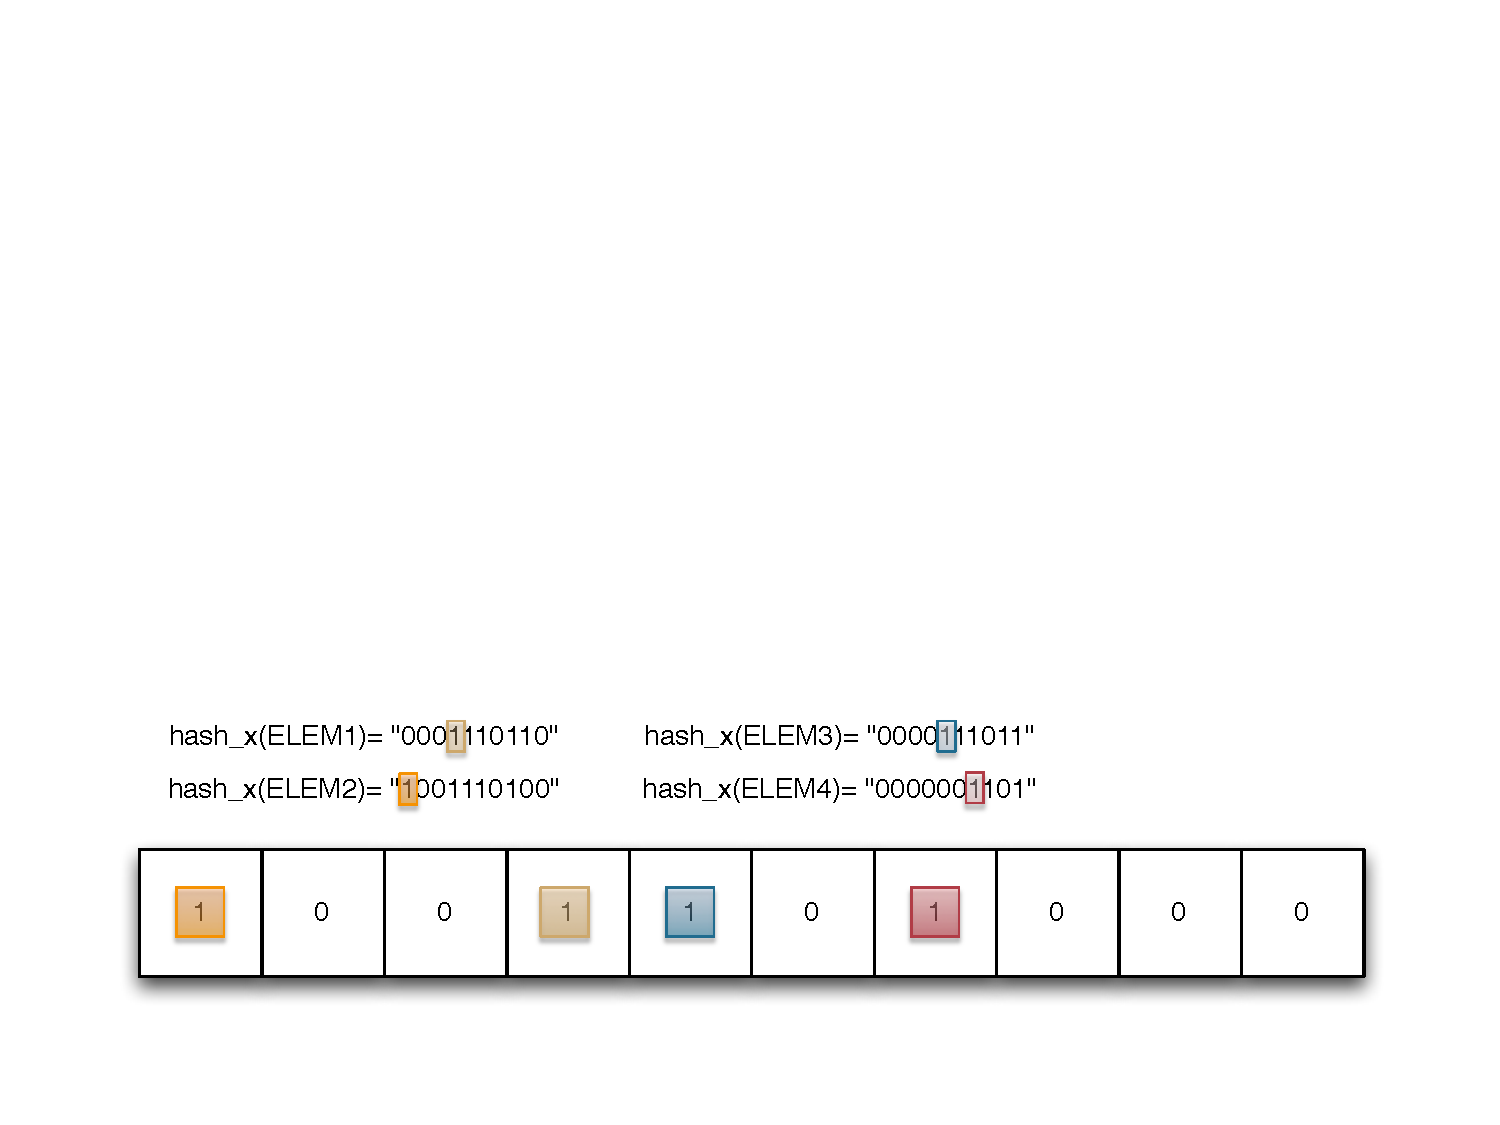
\includegraphics[width=\textwidth]{images/hash_sketch.png}
  \caption{Insertion of an element into a (Hyper)LogLog Sketch}
  \label{fig:hyperloglog_sketches}
\end{figure}

Linear Counting (LC) Sketches \cite{Whang:1990uh}, on the other hand,
use a single bit array/sketch. This sketch is initialized with $0$s.
When an item is to be inserted, its hash value is used to calculate an
index within the sketch, which is then set to $1$. To calculate the
estimate of the number of different items, the algorithm has to use
the fraction of empty sketch entries. In order to obtain this value,
it counts the number of empty sketch entries (the number of $0$
entries in the sketch) and divides it by the total size of the sketch.
Their name comes from their linear space complexity $O(Nmax)$ (where
$Nmax$ is the maximum number of different elements the sketch can
hold), i.e. their size grows linearly with the number of distinct
elements they can hold. Compared to (Hyper)LogLog Sketches, LC
Sketches' space complexity is a drawback, specially for multisets with
large numbers of distinct elements. However, LC Sketches are easier to
implement and also provide better estimates in multisets with a small
number of distinct elements.

Both RIA-DC and RIA-LC Sketches are based on the Linear Counting
Sketches. While RIA-LC can be seen as a slightly improved/simplified
version of Linear Counting Sketches, RIA-DC Sketches have the unique
ability to merge sketches of different sizes. However, this ability
comes with a price. RIA-DC Sketches assume that there is no overlap of
elements belonging to different sketches, meaning that if we merge two
different RIA-DC sketches with elements in common, those elements will
be counted twice in the final aggregate.

It is also worth noting that all the ``observables'' i.e. bit
array(s) used by the above algorithms are order insensitive.
This means that the order in which the elements are inserted does not
affect the output of the estimator functions.
\subsection{Bloom Filters}
\label{sec:bloom_filters}


\subsection{Vector Clocks}
\label{sec:vector_clocks}

%%% Local Variables: 
%%% mode: latex
%%% TeX-master: "../thesis"
%%% End:  % Chapter 2
\chapter{Collaborative Gate Counting}
\label{cha:gate-counting}

In this chapter, we tackle one of the most common forms of urban
sensing: counting unique visitors across multiple gate counters to
measure the number of people across the urban setting.

\section {Motivation and System Model}
\label{sec:motivation}

Bluetooth scanners register the Bluetooth addresses, 48-bit MAC, of
the devices that have been sighted. The Bluetooth device address is a
48-bit MAC format address that uniquely identifies each Bluetooth
device. Some devices are able to switch between multiple Bluetooth
addresses, but for most cases this will be a reliable and permanent
unique identifier for sighted devices and by extension to the
respective owners. A single scan of nearby devices is not in itself
much of a problem. However, a systematic registration of Bluetooth
sightings, especially when done at multiple locations, has the
potential to become a large scale tracking system given the personal
nature of most Bluetooth devices. Relatively simple processes can be
put in place to detect the presence, movements and patterns of
individuals. Concerning anonymity, the absence of a public record
mapping Bluetooth addresses to specific individuals is nothing but a
fragile barrier. To track a specific individual, it would suffice to
intersect the Bluetooth addresses from some of the places she has
visited. Eventually, all that would have been left is a single
Bluetooth address which could then be used to easily track that person
from that moment on. To prevent cases like this, a privacy preserving
approach should avoid permanent storage and dissemination of Bluetooth
addresses or of any other information that could uniquely identify an
individual.

Our Gate Counting scenario assumes the existence of a large set
of heterogeneous and autonomous Bluetooth nodes. We use the terms
\emph{node} and \emph{scanner} interchangeably throughout this document.
Conceptually, a gate is a virtual line across a street, and gate
counting is the process of counting the number of people crossing that
line. Each Bluetooth node is modeled as a gate counter that counts the
number of unique Bluetooth addresses observed during a certain period.
% The use of Bluetooth as an enabling technology to establish the flows
% of people it not a new concept. There are several examples, be it
% within a city~\cite{Oneill:2006vq}, outdoor
% festival~\cite{versichele2012use} or shopping mall
% ~\cite{millonig2008shadowing}.

A Bluetooth-based gate counter does not really count all the people
passing-by, but only those who are carrying discoverable Bluetooth
devices. Still, this is enough to make a reasonable correlation, using
baseline data to estimate the overall traffic. A gate counter should
recognize subsequent sightings of the same entity. In a gate counting
scenario, repeated sightings of the same device can be very common,
not only because people can be passing by multiple times, but also
because of persistent devices. Instead of scanning through a line,
Bluetooth discovery is actually performed in an area and thus any
device in that area, possibly in nearby buildings, would be repeatedly
discovered. Results from empirical studies with known static and
transient devices suggest that a transient device typically appears
for up to 90 seconds while it crosses a gate \cite{Oneill:2006vq}. A
proper gate counting process would thus need to account for this and
filter persistent devices.

A gate counter should also be able to answer questions like ``how many
different people were seen in a given gate in the last 24 hours?'' or
``what was the number of visitors of an amusement park during visitors
peak hours?''. To comply with this requirement, gate counters should
be able to distinguish its readings over time.

The main challenge, however, is how to enable collaborative counting
between multiple independent gate counters, while providing
appropriate privacy guarantees as well as low communication costs. To
be able to count unique entities, we need to identify multiple counts
of the same entity at different nodes, to make sure that the same
device sighted at two different gates will be counted only once.
Imagine, for example, a city festival with multiple gate counters
operating at various locations to count the number of visitors to the
festival. The simple sum of individual gate counts would clearly
overestimate the number of people since many of them would be spotted
at multiple gates. Thus, we need some technique that works across
multiple gate counters and is able to provide an aggregate count of
the unique devices that have been spotted in the entire set
of gate counters. Comparing the plain addresses observed at different
gates would immediately solve this problem, but as we have seen, it is
not suitable for privacy preservation.

\subsection{Objectives}
\label{sec:objectives}

In this chapter, we explore the use of stochastic summarizing
techniques as a privacy preserving approach to enable Bluetooth-based
gate counting of unique entities across multiple nodes. The objective
is to assess the extent to which these techniques are able to address the
specific requirements of this distributed gate counting model, and
inform the design of large scale Bluetooth sensing systems.

Having identified the sensing requirements for this scenario we have
established a number of key criteria for assessing the various
alternatives. Using those criteria, we have conducted an
experimental study in which we compared how multiple types of
stochastic summarizing techniques would behave across multiple
variants of our gate counting scenario. The results provide a strong
foundation for the development of these large scale Bluetooth sensing
infrastructures, identifying major trade-offs and the implications of
key factors such as cardinality and support for merge operations.

% \section{Probabilistic counters for privacy-enhanced gate counting}
% \label{sec:techniques}
% % A common strategy in privacy-enhancing techniques is to reduce the data
% % collected to what is absolutely needed for a particular purpose. In this gate
% % counting scenario, we need to count devices and the ability to check if a
% % particular device has already been counted before. Moreover, we need to be able
% % to do this across a set of autonomous nodes. This means that we are not
% % interested in information about the number or duration of sessions that each
% % device generates at each gate.
% %we may want to know on which gate set a particular device has been seen, we do
% %not need to know the specific sequence through which the device has been seen at
% %those locations.

% Probabilistic counters provide an interesting solution to this problem. They are
% flexible enough for estimating the overall number of unique sightings with some
% controllable accuracy, without ever keeping the plain Bluetooth addresses.


\section{Criteria}
\label{sec:Criteria}

This section tests some of the techniques mentioned in Section
\ref{sec:algorithms_and_data_structures}, namely LogLog Sketches
\cite{Durand:2003tc}, HyperLogLog Sketches \cite{Fusy:2007um}, LC
Sketches \cite{Whang:1990uh}, RIA-LC Sketches,
\cite{Fan:2008wl,YaoChungFanArbeeLPChen:2010to}, RIA-DC Sketches
\cite{YaoChungFanArbeeLPChen:2010to}, Bloom Filters~\cite{Bloom1970}
and Scalable Bloom Filters~\cite{Almeida2007}.

These techniques where picked because they provide an interesting
solution to the gate counting problem. Probabilistic counters are
flexible enough for estimating the overall number of unique sightings
with some controllable accuracy, without ever keeping the plain
Bluetooth addresses.

The requirements identified in section \ref{sec:motivation} boil down
to three important criteria: \textbf{accuracy}, \textbf{size} and
\textbf{aggregation}. These criteria were used in the evaluation the
proposed techniques.

%In the rest of this section we talk about the
%remaining criteria as well as of their respective requirements and analyze
%each technique regarding the aforementioned criteria.

% Processing power SHA1 - Energy Comparison of AES and SHA-1 for Ubiquitous
% Computing

\subsubsection{Accuracy}
\label{sec:accuracy}

With this criterion we want to evaluate the accuracy of the
techniques, their ability to count multiple sightings of the same
device only once, and the quality of their estimators. To do so, we
stipulated the maximum standard error for each technique. In this case
after setting it to  $5\%$, we measured for all % desvio padrão
techniques the relative error (root mean square error) for a range of
cardinalities, whose average of 100 runs is shown in
Fig~\ref{fig:accuracy}.

\subsubsection{Size}
\label{sec:size}
The size of the techniques is an important factor. The less space the
technique requires, the lower will be both the costs of communication
between BT scanners and their memory requirements.

Regarding this criterion, we have 2 fundamentally different
types of techniques: dynamic techniques which consist of Scalable Bloom
Filters and static techniques comprising the rest. Static
size techniques are techniques whose size is set at the time of creation and
cannot be changed afterwards. This means that we must know the maximum
number of unique devices to count before hand, or at least, we must be able
to assume an upper bound for that number. Dynamic techniques on the other
hand don't have this drawback because they can adjust to withstand
arbitrarily large cardinalities. In practical terms this means that for
static size techniques, once we create an instance with a certain capacity
it is not possible to change that capacity afterwards, while for dynamic
techniques there is no such constraint.

To further help us in our analysis, we can look at Figure
\ref{fig:size_benchmark}. Figure \ref{fig:bits_element} depicts the
number of bits per unique element that each technique requires along a
range of cardinalities. Figure \ref{fig:size} shows the total size
spent by each technique to store a given number of distinct elements.

\subsubsection{Aggregation}
\label{sec:mergeAbility}

The ability to merge counts is crucial for scenarios with multiple
gates. It is a key ingredient for obtaining the \emph{aggregate
 number} of individuals in a set of gates. The merge operation
(Figure \ref{fig:merge}) consists in either a bitwise OR operation
(Bloom Filters, Linear Counting, RIA-DC and RIA-LC sketches) or in a
\emph{max} operation (HyperLogLog and LogLog sketches) of structures
that make each gate's counter. In order to merge several gate
counters, there are 2 conditions that must be met: all counters must
be instances of the same technique and every instance must have the
same parameters and capacity (equally sized bit arrays). Meeting these
conditions ensures that the same unique device will mark the same
positions in the several gate counters it crosses. Therefore after
merging the counters, it is possible to obtain the aggregate number of
unique elements without counting the same device repeatedly (Figure
\ref{fig:gate_counter_aggregation}).

\begin{figure}[htb]
\subfigure[\emph{max} Merge- used by LogLog and HyperLogLog Sketches]{
\label{fig:merge_hll}  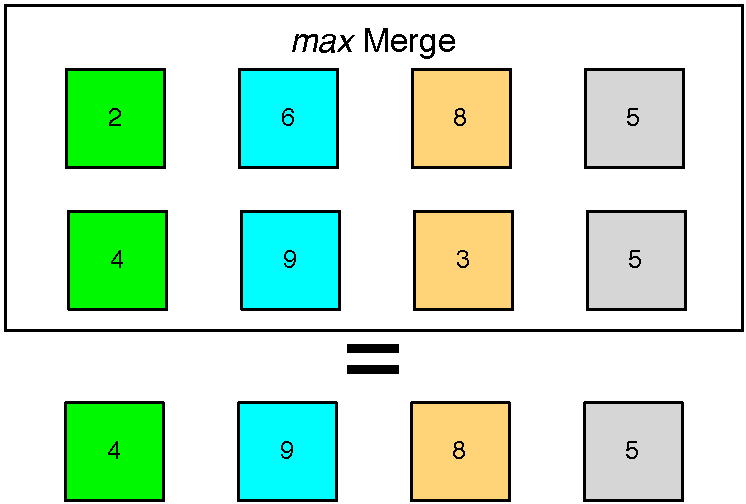
\includegraphics[scale=0.50]{images/merge_max.pdf}
}
\subfigure[Bitwise OR Merge - used by Bloom Filters, RIA-LC, RIA-DC and
LC Sketches]{
 \label{fig:size}  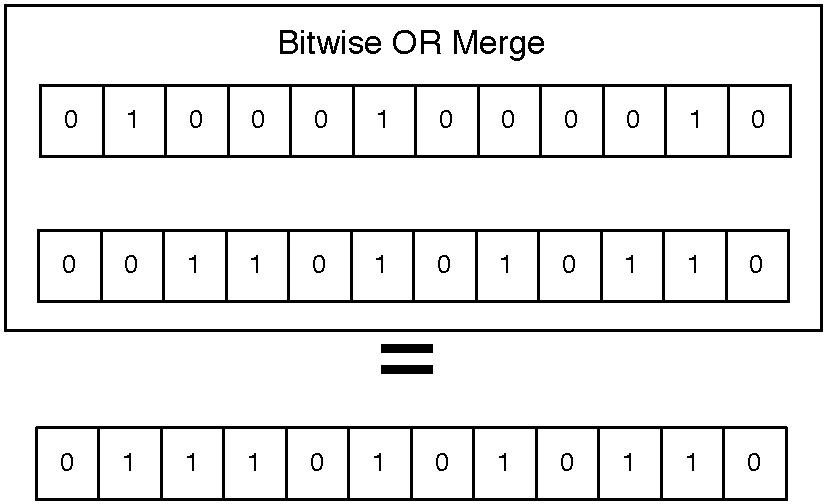
\includegraphics[scale=0.50]{images/merge_or.pdf}
}
\caption{Different Merge Approaches}
\label{fig:merge}
\end{figure}

\begin{figure}[htb]
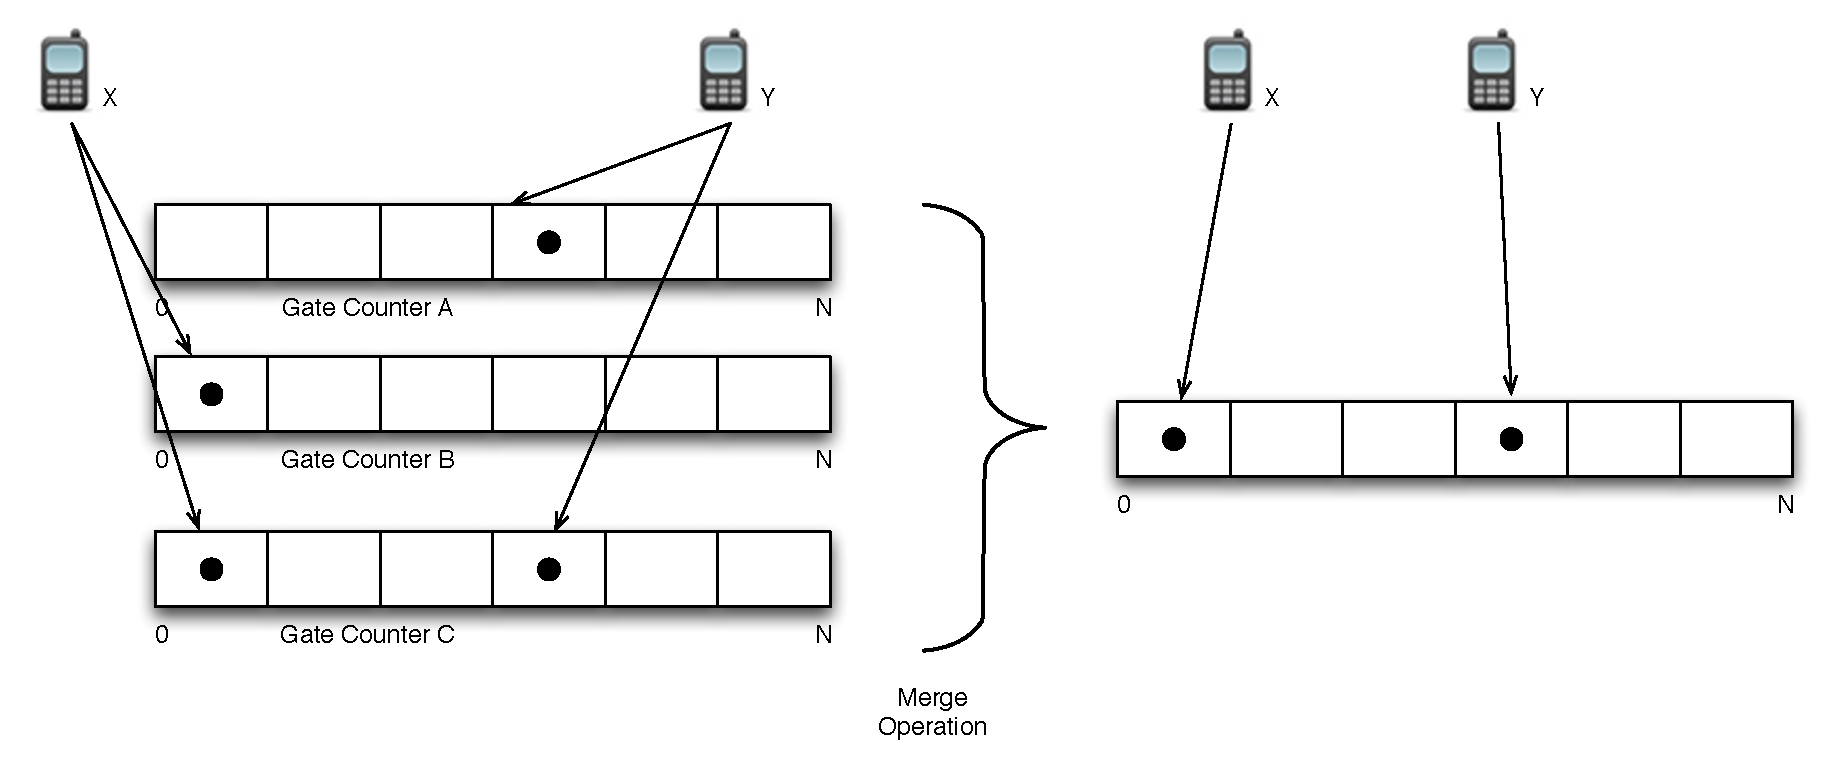
\includegraphics[width=\textwidth]{images/merge.pdf}
\caption{Gate Counter Aggregation - repeated devices appear only once }
\label{fig:gate_counter_aggregation}
\end{figure}

With the exception of Scalable Bloom Filters and RIA-DC sketches, all
the techniques presented here have the ability to merge, and therefore
will not count the same device more than once in aggregate
counts. Scalable Bloom Filters lack the ability to merge because their
size varies dynamically with the number of unique elements, therefore
we cannot guarantee that the same unique device will set the same
positions for different filters. RIA-DC sketches might not provide
accurate aggregate results since the estimator considers there is no
overlap of elements between the different counters.

Aggregation is also important as a mean for answering time related
questions like ``how many different people were seen in a given gate
in the last 24 hours?'' or ``what was the number of visitors of an
amusement park during visitors peak hours?''. To answer these types of
questions, it must be possible to distinguish/segment counter readings
over time. This can by accomplished by sensor nodes periodically
making a copy of their counters followed by a reset. Those copies will
keep the information about the unique devices sighted during a certain
time period. For example, considering that the rate at which counters
are saved and reset is 1 hour, the former question could be answered
by merging the 24 last saved counters. To answer the latter, we would
need to merge the copies made during peak hours at the various nodes
in the park.

To save some space, we can use different time granularities. For
instance, we can merge all unique counters saved during a day and
obtain the aggregate count for the day, merge the counters from the
last 7 days and get the aggregate count for the week, and so forth. We
just need to keep in mind that because of the merge restrictions, the
size of the counter that stores the unique number of devices sighted
during an hour has to big enough to fit the number or unique devices
seen during the entire week.

As we can see, both \emph{time segmentation} and \emph{aggregate counting}
are in fact variations of the same problem, which can only be solved with
techniques that support merging.

\begin{figure}[htb]
%\centering
\subfigure[Upper bound $10^2$]{
\label{fig:accuracy0_1k}  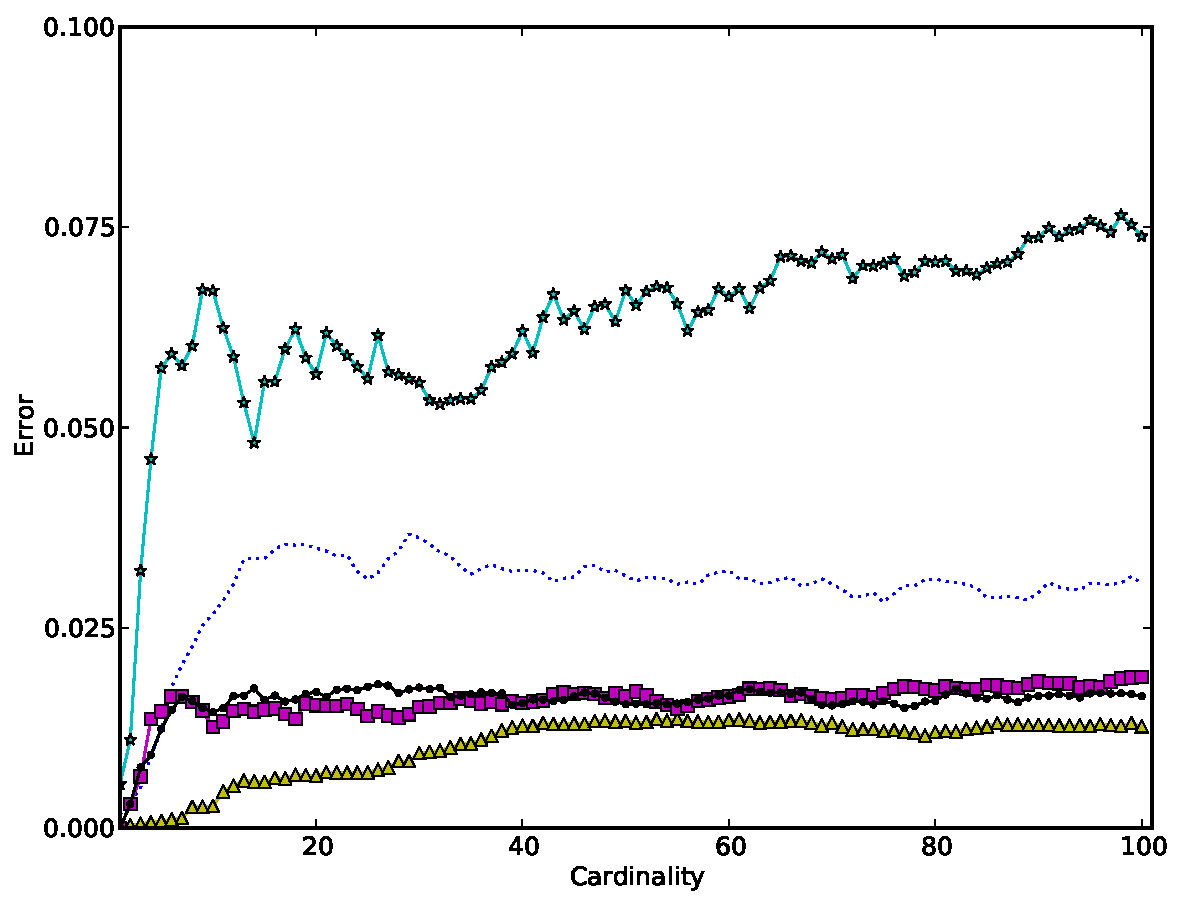
\includegraphics[scale=0.35]{images/0_1k100xAcc.pdf}
}
\subfigure[Upper bound $10^3$]{
 \label{fig:accuracy1k}  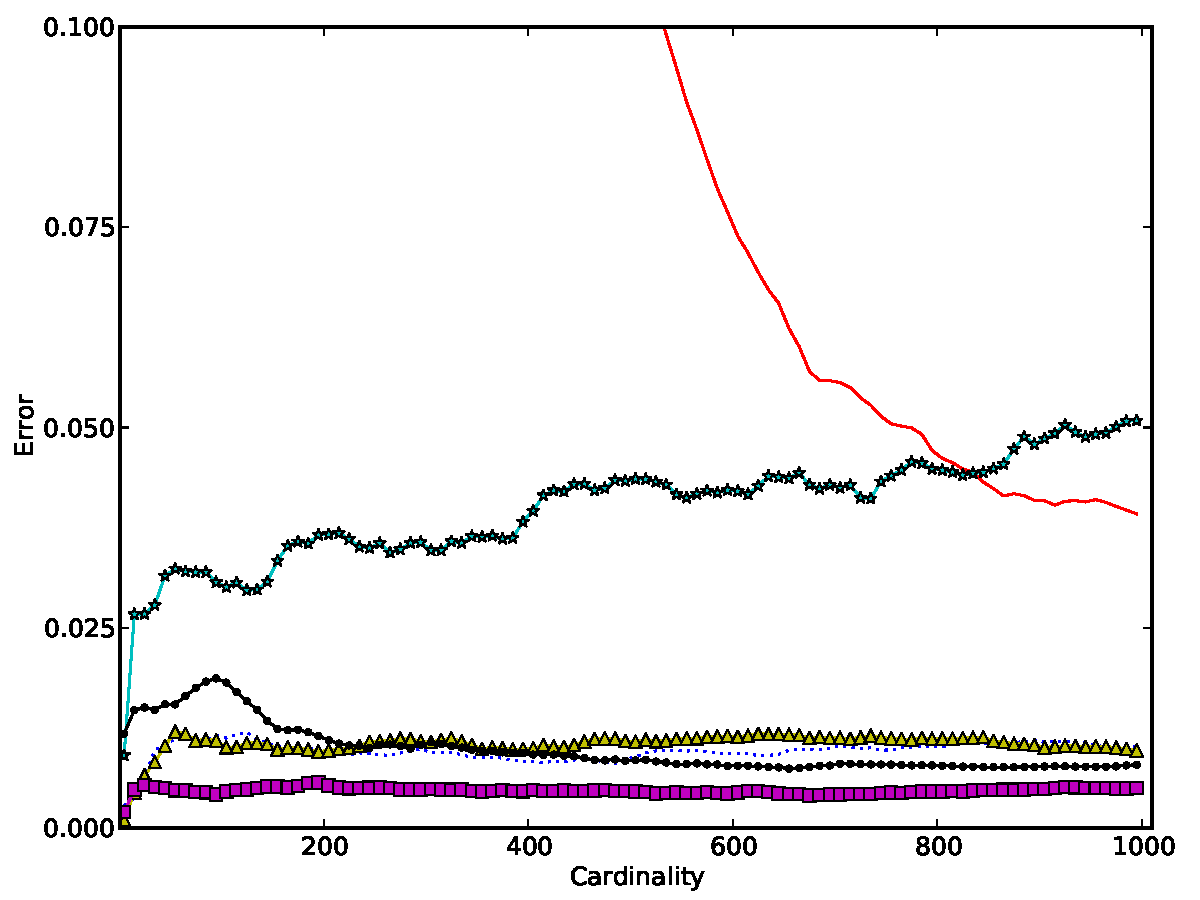
\includegraphics[scale=0.35]{images/1k100xAcc.pdf}
}
\subfigure[Upper bound $10^4$]{
  \label{fig:accuracy10k} 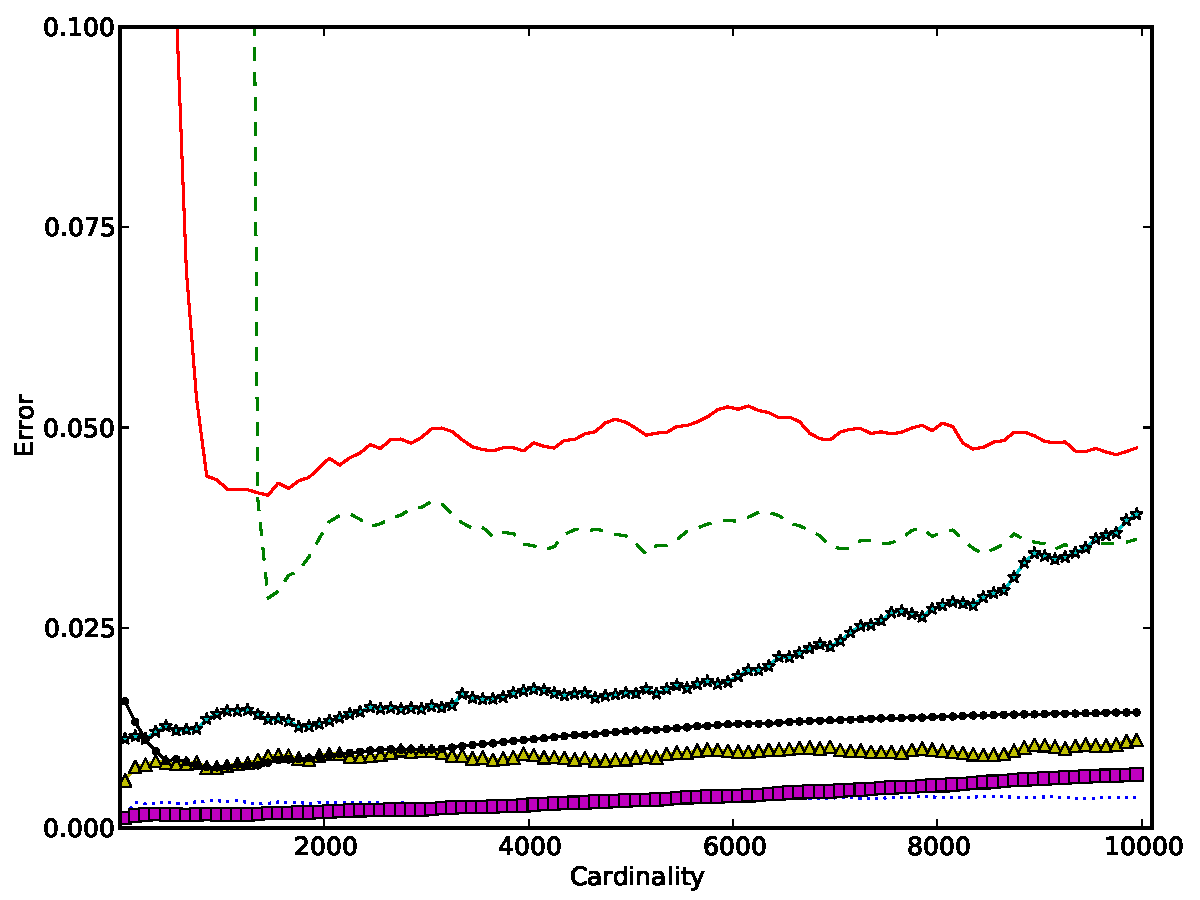
\includegraphics[scale=0.35]{images/10k100xAcc.pdf}
}
\subfigure[Upper bound $10^5$]{
  \label{fig:accuracy100k} 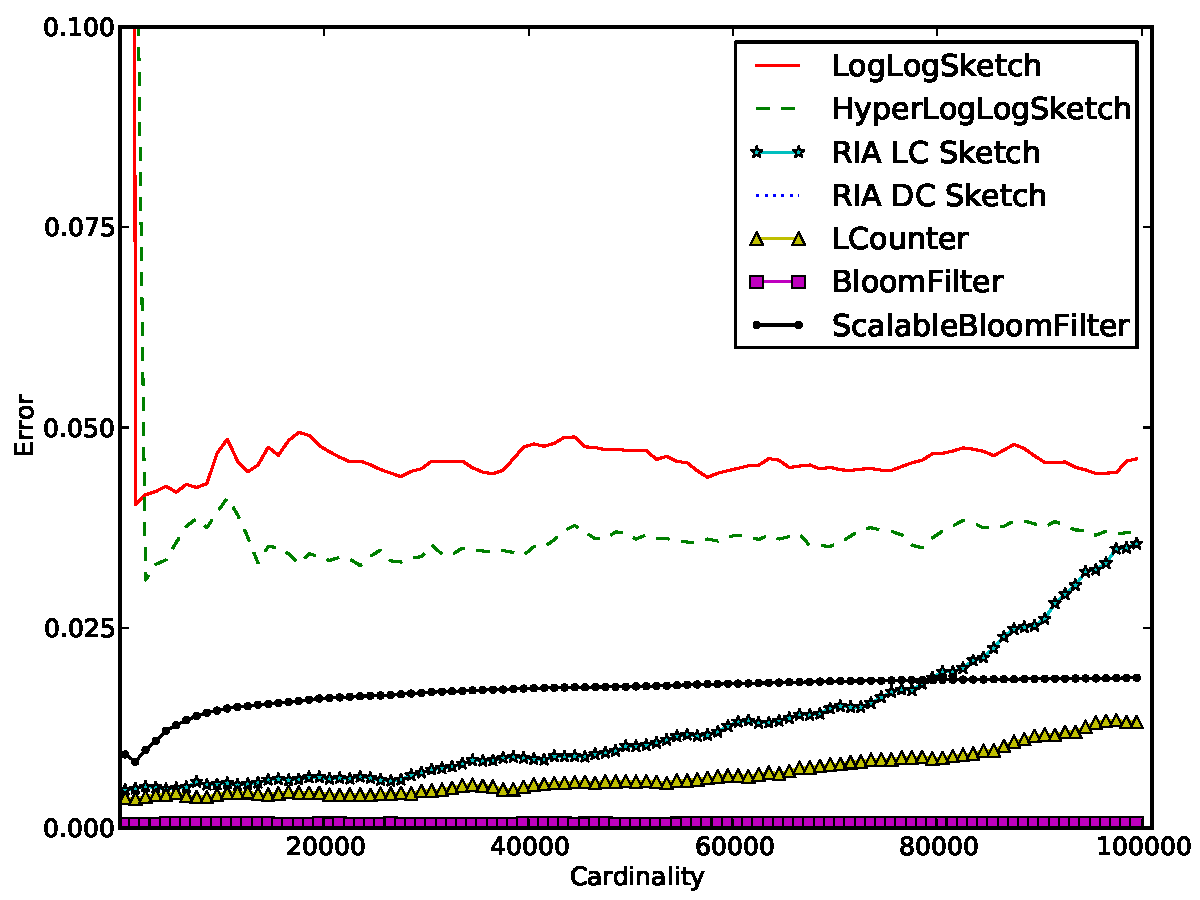
\includegraphics[scale=0.35]{images/100k100xAcc.pdf}
}

\caption{Relative error of the several techniques using various upper
  bounds. Average of 100 runs.}
\label{fig:accuracy}
\end{figure}

\begin{figure}[htb]
%\centering
\subfigure[Number of bits per element used by each technique at different cardinalities]{
\label{fig:bits_element}  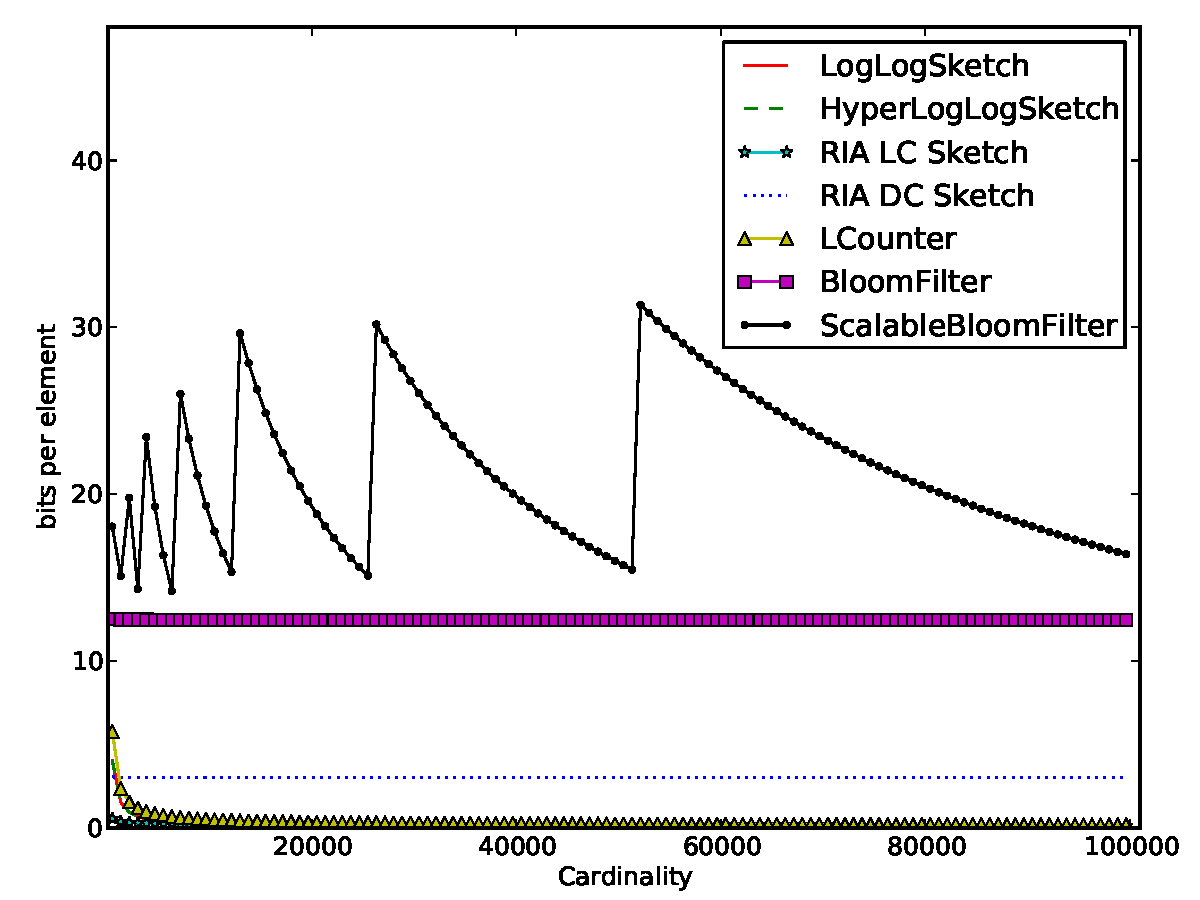
\includegraphics[scale=0.35]{images/bits_per_element_100k.pdf}
}
\subfigure[Size of the several techniques for different cardinalities]{
 \label{fig:size}  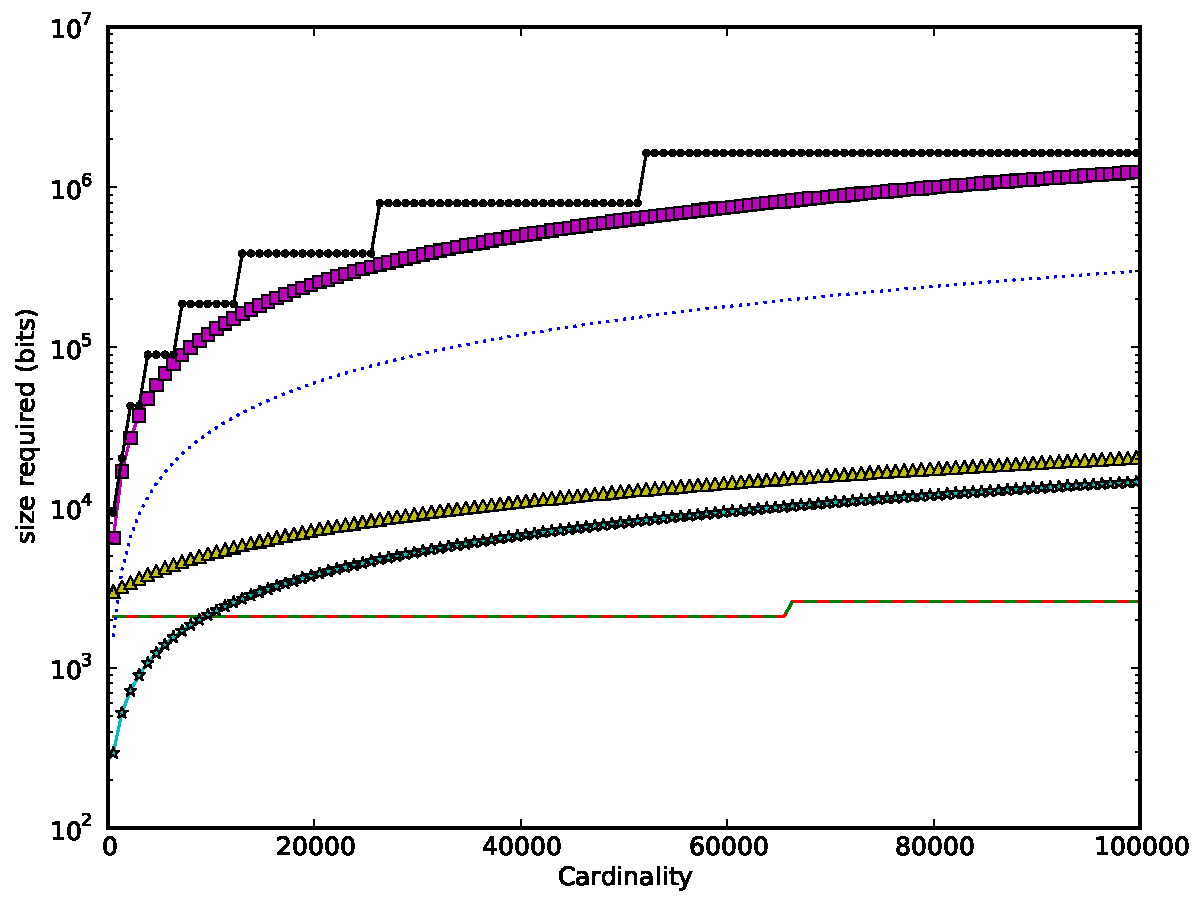
\includegraphics[scale=0.35]{images/size_100k.pdf}
}
\label{fig:size_benchmark}
\caption{Size benchmarks}
\end{figure}

\section{Evaluation}
\label{sec:evaluation}
Using the results from our benchmark\footnote{Our Benchmark was built
  in Python, including the implementation of the several algorithms,
  with the exception of Bloom Filters where we used Jay Baird's
  implementation.} shown in figures \ref{fig:accuracy} and
\ref{fig:size_benchmark} and having explained the
different criteria we can now analyze each one of the techniques.

\subsubsection{Standard and Scalable Bloom Filters}
Both techniques provide a good accuracy for all the cardinalities
tested, never surpassing the stipulated relative error. Figure
\ref{fig:accuracy} confirms both these facts. However, looking at
Figure \ref{fig:size_benchmark} we can confirm that in regard to
space, they are the most expensive techniques of all. This extra cost
in terms of space stems from their query membership ability. Figure
\ref{fig:size_benchmark} also highlights the incremental nature of
Scalable Bloom Filters. Each time the filter gets full, a new Bloom
Filter is created, increasing the size of the technique. This explains
the seemingly strange behavior of the technique. Both these techniques
are also the most computationally expensive of all in terms of
insertion complexity.

\subsubsection{LogLog and HyperLogLog Sketches}
As depicted by Figures \ref{fig:accuracy0_1k} and
\ref{fig:accuracy1k}, these techniques have very low accuracy for
small cardinalities ($\lesssim 1800$). Apart from this issue, they are
the best suited techniques for large cardinalities due to their
logarithmic growth in size. As shown in Figure \ref{fig:size}, for
numbers of distinct elements above 10000, these are the most efficient
techniques in terms of space. Between the two, HyperLogLog sketches have
the advantage of being more accurate and of having a smaller
variance. Regarding insertion complexity, these techniques are less
expensive than Bloom Filters, but more expensive than the LC Sketches
based ones.

\subsubsection{LC Sketches, RIA-LC Sketches and RIA-DC Sketches}
Spending only a little more memory than LogLog Sketches, LC Sketches
do not suffer from poor accuracy in smaller cardinalities, they have
an all around good accuracy just like Bloom Filters. LC Sketches are
a good all around technique. Being based on Linear Counting Sketches,
it is no surprise that RIA-DC and RIA-LC Sketches also have good
accuracy results. Furthermore and like their ancestor, they also
achieve good results in the bits per element ratio. These techniques
are also the ones with the smallest complexity in
terms of element insertion. \\ \\

Taking into account all that has been said, there are a few
conclusions to be drawn. For scenarios where we cannot make
assumptions on the maximum number of elements to count, we have to use
Scalable Bloom Filters. For scenarios where there is a big discrepancy
between the cardinalities of different counters and where the
existence of repeated elements outside each counter can be neglected,
RIA-DC Sketches are probably the best choice. For scenarios with very
large cardinalities HyperLogLog Sketches are probably the correct
choice since they are the most space efficient technique.  Considering
the expected most common scenarios, where we need accurate aggregate
counts and where there is the possibility of counters with low
cardinalities, the choice falls either within Linear Counting Sketches
or RIA-LC Sketches. We prefer the latter since it is a slightly
simplified version of the former.

As a final remark, we should emphasize the fact that all the
techniques discussed in this chapter are more efficient in terms of
space than storing each unique device's 48 bit MAC address (check
Fig.\ref{fig:bits_element}).

\section{Summary}
\label{sec:gc_summary}
Bluetooth devices are pervasive in most societies and the number of unique
Bluetooth sightings is an adequate proxy for the number of actual individuals
present. The trivial approach of collecting and counting the set of detected
Bluetooth MAC addresses is not adequate, in most settings, both in terms of
privacy concerns, system scalability and adequacy to devices with limited
memory.

In this chapter we described and benchmarked a set of stochastic summarizing
techniques that can be applied to the gate counting problem. By using these
techniques our approach ensures the privacy of the users since Gate Counters
don't store any extra raw information, i.e., the raw information that
they keep at any given moment is also present in the Bluetooth network.

Furthermore, the analysis of these techniques and their trade-offs
should help to determine the most adequate solutions for a specific
gate counting scenario. % We also hope to have motivated the community
% to the relevant role of stochastic counting techniques in privacy
% preserving gate counting.

%%% Local Variables:
%%% mode: latex
%%% TeX-master: "../thesis"
%%% End:
 % Chapter 3
\chapter{Causality Tracking}
\label{cha:causality-tracking}
This chapter, addresses the use of Bluetooth sightings as a way to
acquire knowledge about the movement patterns of people. To do so, we
propose a new technique with adjustable accuracy capable of
representing the causality relation between visited places. 

\section{Motivation and System Model}
\label{sec:ct-motivation}

The use of hash functions is often suggested as a data sanitation
technique in which the Bluetooth address is replaced by a digest from
which it is not be possible to recreate the original address. However,
this is also not suitable for large scale BT sensing, as it would be
possible, even with minimal information about someone, to identify the
respective digest, and from that point onward, the digest would again
function as a unique identifier (pseudonym).

There are examples, such as the Netflix
case~\cite{DBLP:journals/corr/abs-cs-0610105} that show how
surprisingly easy it can be to personalize information that was being
proposed as anonymous (\emph{quasi-identifier}
~\cite{bettini2005protecting}) simply by adding some basic additional
knowledge to the system. This is also visible in other
domains~\cite{Ohm:2010tc}. Therefore, the systematic registration of
Bluetooth sightings done at multiple locations constitutes a privacy
threat in that it allows the creation of a surveillance system for
people.

The use of Bluetooth as an enabling technology to establish the flows
of people is not a new concept. There are several examples, be it
within a city~\cite{Oneill:2006vq}, outdoor
festival~\cite{versichele2012use} or shopping mall
~\cite{millonig2008shadowing}.

The model in which we base our work assumes the existence of a network
of heterogeneous and autonomous nodes that collaborate in the
tracking process of Bluetooth devices. These nodes may have access to
various types of information about the devices: their MAC address, the
timestamp of the sighting, the type of Bluetooth protocols supported
by the devices, among others. 

Similarly to Gate Counting scenario in Chapter
\ref{cha:gate-counting}, there is the possibility of using preexisting
resources (nodes). As a consequence, our model does not impose
restrictions on the type of information registered by the
scanners. The nodes will continue to perform the same functions they
did before as a part system. Our concern is to the information that
might be exchanged by the nodes in the context of collective tracking
and to the privacy risks that might ensue such as the ability
to accurately follow the movement of a device and therefore of its
respective owner.

In their everyday life and depending on their specific needs, people
visit several different places. For instance, a person $P_1$ wants to
buy a new laptop. To do so, she visits store $S_1$ which does not have
the model she wants. She then visits store $S_2$ which is out of
stock and afterwards store $S_3$ where the price is a little
steep. She ends up buying the laptop in store $S_4$. To represent this
behavior we introduce the concept of \emph{mobility traces}. A
mobility trace is simply the representation of the places visited in the
order by which they were visited. In this specific case, the mobility
trace of $P_1$ is $T_{P_1}=\{S_1,S_2,S_3,S_4\}$. Our mechanism
\emph{Precedence Filters}, allows the recording of information
relative to the individual traces of people, in a manner compatible
with plausible deniability. That information can later be
processed/mined to obtain more accurate data about the habits of the
aggregate of all individuals. For instance, in this example, the order
in which the stores where visited might be an indicator of their
reputation/popularity.

A common strategy that seeks to strengthen privacy is the restriction
of captured data to just the essential. In our specific case, the goal
is the detection of movement patterns between nodes. As such, the
ability to detect the same device on different nodes is paramount. To
minimize the amount of information collected, we can ignore
information such as the duration of the sightings, the timestamp in which
they occurred, the device name, supported Bluetooth protocols,
among others. We just need the device's MAC address.

Whenever a device is sensed, the sighting node records that event
locally. This information is then used in the computation of device
transitions between the system's multiple nodes. The place where that
computation takes place depends on the system's architecture. In a
centralized system, the computation has to be done in the server since
only it has enough information to do so. Each node only shares its
local information with the server. On the other hand, with a
decentralized architecture, the processing can be done locally by the
nodes. The local information each node possesses is shared with the other
nodes, thus allowing all the nodes to have access to the same
data. Both models have advantages and disadvantages. For instance, the
centralized approach is not fault tolerant, if the server crashes the
tracking system stops working. This does not happen in the
decentralized approach given that the same information is stored in
multiple nodes (redundancy). The system can keep on working even if
some of the nodes fail. Compared to the centralized version, the
decentralized model also has greater availability, result of the
information redundancy. However, as a consequence of the exchange of
information between all the nodes, the decentralized scenario has
a bigger burden on the network when compared to the centralized one. 


In order to achieve the goal we set ourselves and taking into account
the constrains presented by our model, our solution is based upon the
following set of assumptions:
\begin{itemize}
\item Even though we cannot make assumptions about how each individual
  node will handle the observed Bluetooth addresses, our solution
  should never require the Bluetooth address or any other information
  that could uniquely identify individuals to ever leave the sensing
  node.
\item No system element should at any given time have all the
  information necessary to accurately determine the path of a single
  individual.
\item The aggregate result that a node can create about the set of all
  visiting devices should be accurate enough to be useful in human
  mobility observation scenarios, e.g. most common paths, similarity
  level between places.
\item There are no communication failures in the system and the
  exchange of information between any two nodes is faster than the
  time it takes for a person to move between them. This ensures that
  the order in which the sightings are recorded is correct, i.e, when
  a person goes from place $A$ to place $B$, node $B$ must already
  have the information that she was in $A$. 
\end{itemize}

\subsection{Objectives}
\label{sec:ct-objectives}
In this chapter, we discuss the use of Bluetooth sightings, captured
by a group of cooperative scanners, with the purpose of obtaining
information about the movement patterns of users. All of this
without compromising their privacy. Particularly, we wish to explore
the application of stochastic summarizing techniques as privacy
preserving approach to Bluetooth Tracking.

The technique presented in this chapter, Precedence Filters (PFs), gives
each Bluetooth scanner the ability to obtain probabilistic information
about the provenance of the detected visitors. This information
concerns the nodes which were visited just prior to the current
scanner. Its accuracy can be adjusted to an uncertainty level
compatible with plausible deniability. This means that it must be
reasonable to believe an individual who denies being in a given place
even if the technique points
otherwise. % Even so, the information about the aggregate of
% all visitors must have enough accuracy to be relevant in the study of
% the group's movement patterns.
However, when considering the aggregate view of all the visits, the
algorithm is able to provide enough accuracy to be a relevant source
of data for Human mobility studies.

\section{Precedence Filters}
\label{sec:precedence-filters}
By applying some of the previously mentioned (Subsection
\ref{sec:vector_clocks}) general constructs of distributed systems to
the mobility sensing scenario, Bluetooth scanners can be treated as
processes and device sightings as state transition events. Precedence
Filters are based upon this idea and provide accurate mobility
information data at a macroscopic level without neglecting individual
privacy.  Precedence Filters can be seen as a vector clock
\cite{Fidge,Mattern} implementation whose difference is the use of
Counting Bloom Filters~\cite{Fan98summarycache:,Mitzenmacher:2002:CBF:581876.581878} (one for each node in the system) by the PFs
instead of integers (one per process) used by vector clocks.

In the decentralized model each Bluetooth node has its own PF and the
nodes communicate with each other upon sighting events in order to
keep their filters updated. On the other hand, in the centralized
approach, each node possesses a simple CBF, whose updates can only be
made through communication with the centralized server. In turn, the 
centralized server maintains an up to date copy of each node's CBF,
i.e. a Precedence Filter.

\begin{figure}
  \centering
  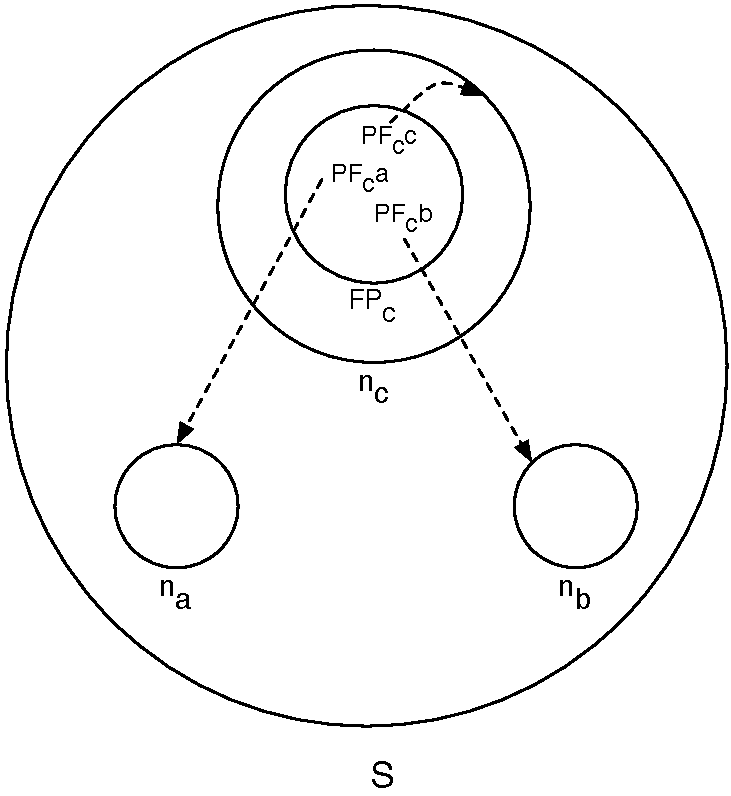
\includegraphics[width=0.60\textwidth]{images/precedence_filters.pdf}
  \caption{Diagram of relevant entities and data structures}
  \label{fig:precedence_filters}
\end{figure}

Our work is based in the decentralized approach. Both our
implementation and the tests we ran are based upon it. So,
from now on, we will be referring to the decentralized version only,
although it is not hard to draw conclusions that apply to the
centralized scenario as well.
With that in mind, Precedence Filters work as follows: supposing we
have a set of Bluetooth scanners (nodes) $S$, each node $n \in S$ has
a Precedence Filter $PF_n$. That PF is in turn composed of a set of
\emph{Counting Bloom Filters}, one for each node $z \in S$. We use
notation $PF_n^z$ to refer to the CBF for scanner $z$ belonging to
$PF_n$, as depicted in Figure ~\ref{fig:precedence_filters}.

All CBFs are initially set to 0, use the same set of hash functions
$K$ and have the same size $M = m * k$ ($k$ is calculated with
equation \ref{eq:optimal_hash_number} and $m$ is calculated with
equation \ref{eq:optimal_slice_size}). This ensures that the same
device is correctly identified across the several nodes (upon
detection it will be mapped to the same indices). Precedence Filters
can also be seen as a matrix where the number of rows is equal to the
number of nodes in the system and the number of columns is equal to $M$.

Each time a node $n$ detects a device $d$, its Precedence Filter
$PF_n$ is updated according to the following set of rules:
\begin{enumerate}
\item Using the set of hash functions $K$, the node $n$ calculates the
  set of indices $I_d$. $I_d$ consists on the output from the $K$ hash
  functions regarding device $d$, $I_d=\bigcup_{f \in K} f(d)$.
\item Node $n$ sends the set of indices $I_d$ to the all other nodes
  in $S$.
\item Each one of the $q$ nodes belonging to $Z$ ($Z = S \backslash
  \{n\}$) replies with a set of tuples $R_q$. $R_q$ contains
  the previously required $I_d$ along with the set of values that each
  of the CBFs belonging to $FP_z$ had stored in those indices,
  $R_q^{I_d}= (i,\{PF_z^x[i]\}) ,\forall i \in I_d, \forall x \in Z$
\item Upon the reception of the replied from the other nodes, $n$
  updates its own indices $I_d$ on the CBFs relative to the other
  nodes with the maximum value received, $PF_n^z[i] = \max(R_q[i][z] \forall
  q \in Z), \forall i \in I_d, \forall z \in Z$
\item Lastly, $n$ updates the indices $I_d$ on its own CBF
  ($PF_n^n$). For each index $i \in I_d, PF_n^n[i] = \max(PF_n^d[i])+1,
  \forall d \in S$. By adding 1 to the maximum value stored in the
  other nodes, the current node ``dominates'' them in the operation
  that returns the causality between the visited places. In other
  words, it is the key to obtaining the order in which the places were
  visited. 
\end{enumerate}

This set of rules allows the precedence filters to record information
about the precedence of the locals visited by a device. Given a set of
indices $I_d$ for device $d$ and any pair of scanners $x$ and $y$, we
say that the sighting of $d$ in $x$ precedes the one in $y$, $x
\leadsto y$ if: 

\begin{center}
\begin{math}
	x\leadsto y \Longleftrightarrow PF_{x}[I_d] < PF_{y}[I_d]
\end{math}
\end{center}
Where $PF_x[I_d] < PF_y[I_d]$ stands for:
\begin{center}
  \begin{math}
    \forall i \in I_d : PF_x^x[i] < PF_y^y[i]
  \end{math}

\end{center}
It is easy to see the similarities with the vector clock description
from Subsection \ref{sec:vector_clocks}. 

Mobility traces, used in our model to describe the behavior of
individuals, characterize a total order between the places
visited. This means that it is always possible to establish an order
between any two elements from the mobility trace. Being based upon the
happens-before relation~\cite{Lamport:1978}, Precedence Filters can
only represent partial orders. In this particular case, for each of
the nodes/locations they can only ``remember'' the last time each
device was sighted. For instance, given the mobility trace
$T_{P_1}=\{S_1,S_2,S_1,S_3,S_2,S_4,S_1\}$ where places $S_1$ and $S_2$
are visited more than once, in the best case scenario PFs can obtain
$T_{P_1}=\{S_3,S_2,S_4,S_1\}$. This is a consequence of the
irreflexivity and antisymmetry properties from the happens-before
relation. However, we can look at this as a feature of Precedence
Filters, a sort of automatic data degradation. It ensures that the
record of sightings for any given device has an upper bound equal to
the number of Bluetooth scanners in the tracking system.

The level of privacy offered by Precedence Filters can be further
customized by adjusting the CFBs' false positive ratio (Equation
\ref{eq:false_positive}). The higher the ratio, the greater the
inaccuracy of the PFs. The occurrence of false positives in the CFBs
results in the appearance of \emph{fictitious transitions}, i.e. the
causal trace obtained from querying the filters, contains transitions
which are non-existent in the original trace. 

Both these properties are what allow individual users to deny the
legitimacy of the data extracted from the Precedence Filters.


\section{Evaluation}
\label{sec:ct-evaluation}

\subsection{Simulator}
\label{sec:simulator}


\section{Synopsis}
\label{sec:ct-synopsis}

%%% Local Variables: 
%%% mode: latex
%%% TeX-master: "../thesis"
%%% End: 
 % Chapter 3
\chapter{Conclusion}
%%% Local Variables: 
%%% mode: latex
%%% TeX-master: "../thesis"
%%% End: 

% \appendix
% \input{appendices/appendixA.tex} % Appendix A
% \input{appendices/appendixB.tex} % Appendix B

% Back matter
\backmatter
\bibliographystyle{plain}
\bibliography{library}
\addcontentsline{toc}{chapter}{\bibname}

\end{document}
